\section{Fuzzy membership function}

A crisp set is defined by a boolean membership function on some property of the considered elements. 
In contrast, a fuzzy set is a set whose membership function ranges between zero and one.
\begin{definition}
    A \emph{membership function} defines a set by specifying the degree of membership of an element from the universe of discourse to the set. 
    A \emph{label} is assigned to the set to provide a reference. 
    Fuzzy sets can also be defined with a variable having discrete values.
\end{definition}
\begin{figure}[H]
    \centering
    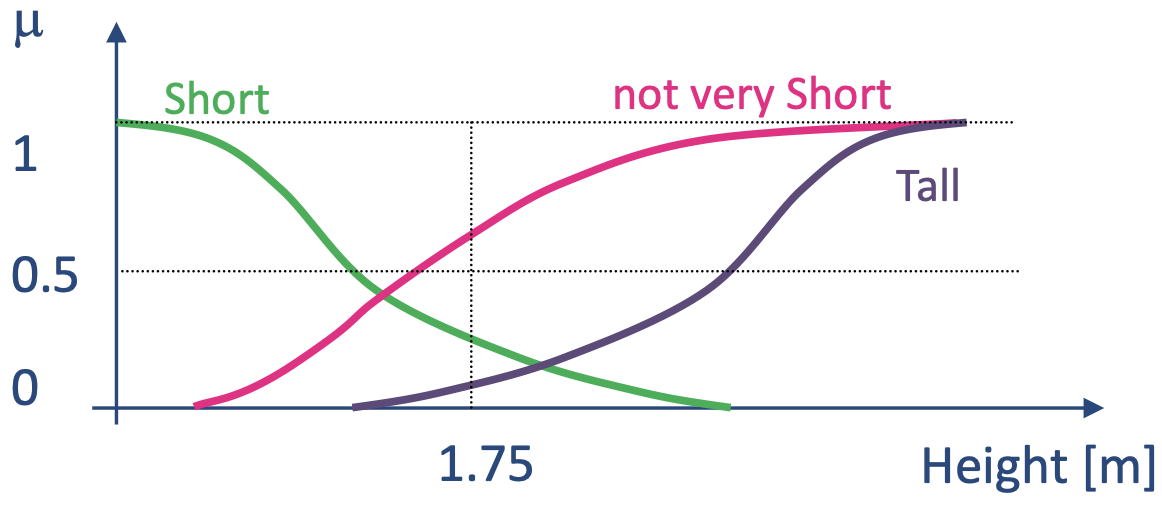
\includegraphics[width=0.4\linewidth]{images/function.png}
    \caption{Example of a membership function}
\end{figure}
To define a membership function, we need to consider the following steps based on the purpose of the model and the available data:
\begin{enumerate}
    \item Select a variable on which the membership function will be defined.
    \item Define the range of the variable.
    \item Identify the fuzzy sets needed for the application and define the labels.
    \item Identify characteristic points for the membership function for each fuzzy set.
    \item Define the shape of the membership function.
    \item Verify the correctness of the membership function.
\end{enumerate}
The shapes of the membership function can be chosen arbitrarily. 
The choice of shape affects the smoothness of the transition between two labels (e.g., a horizontal shape results in an immediate transition within intervals).
\begin{figure}[H]
    \centering
    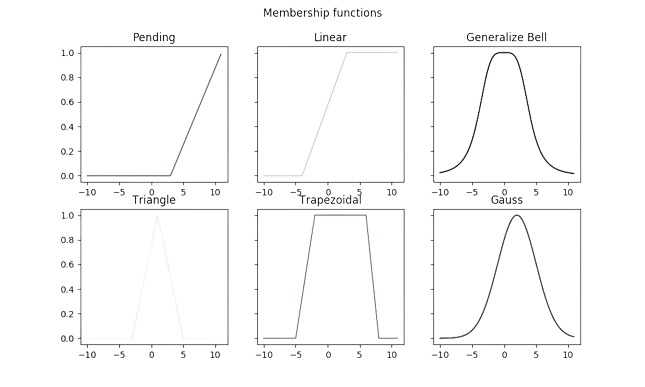
\includegraphics[width=0.75\linewidth]{images/shape.png}
    \caption{Possible shapes for a membership function}
\end{figure}
\begin{definition}
    A set of fuzzy sets that fully covers the universe of discourse is called a \emph{frame of cognition}. It has the following properties:
    \begin{itemize}
        \item Coverage: each element of the universe of discourse is assigned to at least one granule with membership greater than or equal to zero.
        \item Uni-modality of fuzzy sets: there is a unique set of values for each granule with maximum membership. 
    \end{itemize}

    A frame of cognition for which the sum of the membership values of each value of the base variable is equal to one is called a \emph{fuzzy partition}.

    The \emph{$\alpha$-cut} of a fuzzy set is the crisp set of values of $x$ such that $\mu(x) \geq \alpha$:
    \[\alpha_\mu(x)=\{x \mid \mu(x) \geq \alpha\}\]
\end{definition}
\begin{figure}[H]
    \centering
    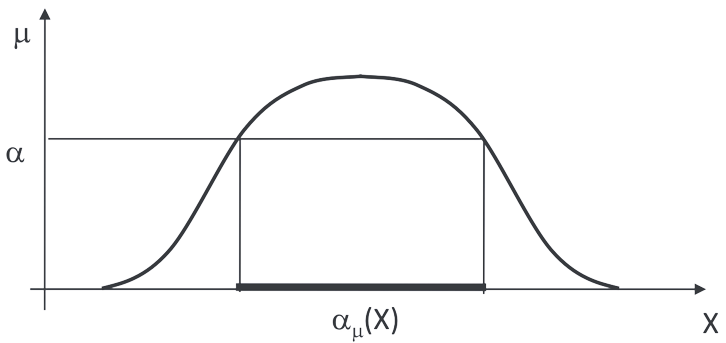
\includegraphics[width=0.4\linewidth]{images/alpha.png}
    \caption{Alpha-cut of a membership function}
\end{figure}
\begin{definition}
    The \emph{support} of a fuzzy set is the crisp set of values $x$ such that $\mu_f(x)>0$. 
\end{definition}
\begin{figure}[H]
    \centering
    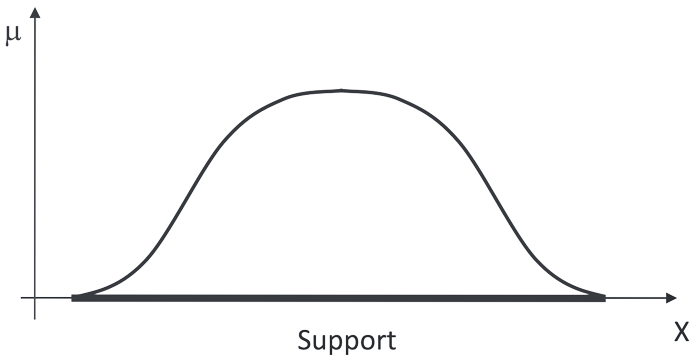
\includegraphics[width=0.4\linewidth]{images/support.png}
    \caption{Support of a membership function}
\end{figure}
\begin{definition}
    The height $h_f$ of a fuzzy set $f$ on the universe $X$ is the highest membership degree of an element of $X$ in the fuzzy set:
    \[h_f(X)=\max_{x \in X}\mu_f(x)\]
    A fuzzy set is considered normal if, and only if, $h_f(X)=1$.
\end{definition}
\begin{figure}[H]
    \centering
    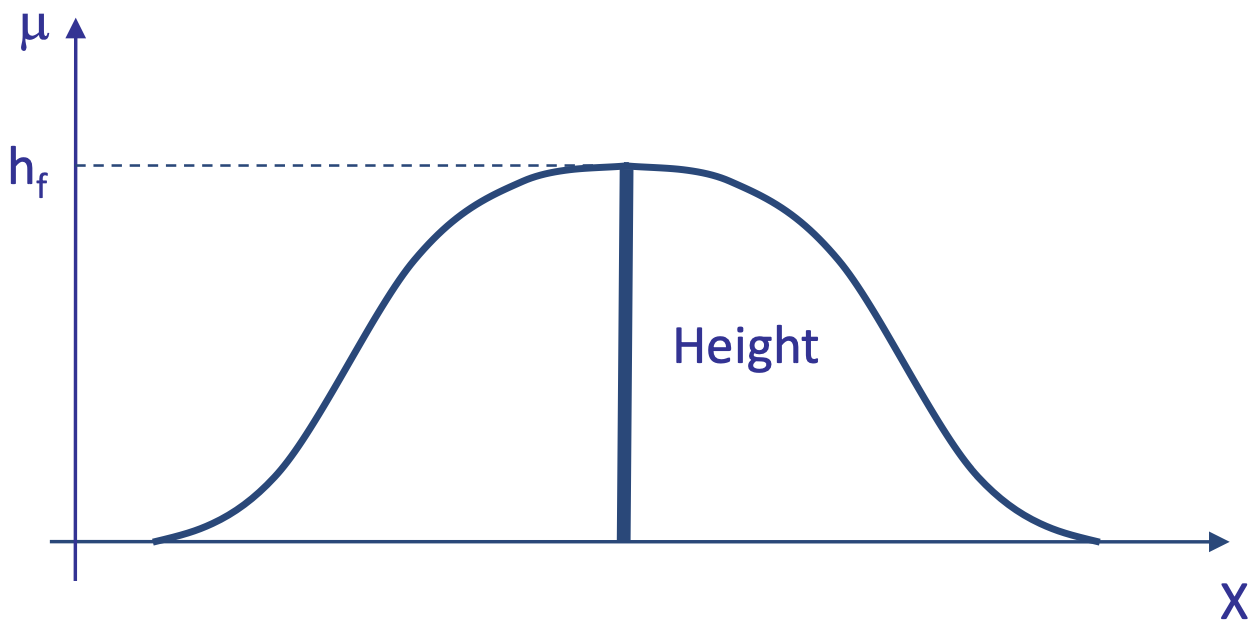
\includegraphics[width=0.4\linewidth]{images/height.png}
    \caption{Height of a membership function}
\end{figure}
\begin{definition}
    A fuzzy set is \emph{convex} if and only if 
    \[\mu[\lambda x_1+(1-\lambda)x_2] \geq \min [\mu(x_1),\mu(x_2)]\]
    for any $(x_1,x_2) \in \mathbb{R}$ and any $\lambda \in [0,1]$.
\end{definition}
\begin{figure}[H]
    \centering
    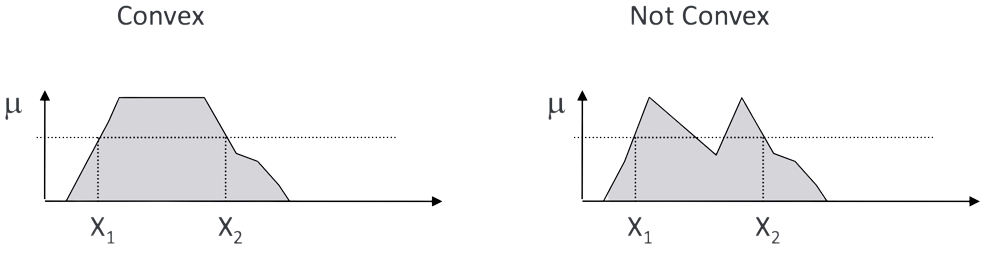
\includegraphics[width=0.75\linewidth]{images/convex.png}
    \caption{Graphical difference between a convex and a not convex set}
\end{figure}
The specific fuzzy sets include "singleton" (a fuzzy set comprising exactly one member) and "interval" (a fuzzy set where all members have a membership value equal to one). 
The available operations on fuzzy sets encompass:
\begin{itemize}
    \item Complement: $\mu_{\bar{f}}(x)=1-\mu_f(x)$.
    \item Union: $\mu_{f_1 \cup f_2}(x)=\max [\mu_{f_1}(x),\mu_{f_2}(x)]$.
    \item Intersection: $\mu_{f_1 \cap f_2}(x)=\min [\mu_{f_1}(x),\mu_{f_2}(x)]$.
\end{itemize}